\documentclass[twocolumn]{article}
\usepackage{graphicx}
%\usepackage{fancyhdr} 
%\usepackage{fancybox}
\usepackage{float}
\usepackage{listings}
\usepackage[colorlinks=true,urlcolor=black,linkcolor=black]{hyperref}
\usepackage[margin=1.0in]{geometry}
\usepackage{multicol}
\usepackage{type1cm}
\usepackage{lettrine}
%\pagestyle{fancy}

%redefines subsections with letters instesad of numbers
%\renewcommand{\thesubsection}{\thesection.\alph{subsection}}

% Center Image Command
\newcommand{\centerimage}[3]{
\begin{figure}[ht!]  
\begin{center} #1
\caption{#2}
\label{#3}
\end{center}
\end{figure}}

\newcommand{\centertable}[3]{
\begin{table}[ht!]  
\begin{center} #1
\caption{#2}
\label{#3}
\end{center}
\end{table}}

\title{\textbf{Branch Predictor and Branch Target Buffer} \\
ECE 486/586 Final Project }
\author{Eric Krause \hspace{1.4in} Bradon Kanyid\\
\url{ekrause@pdx.edu} \hspace{1in} \url{bradon@kanyid.org}}

\begin{document}
\twocolumn[
  \begin{@twocolumnfalse}
    \maketitle
    \begin{abstract}
      ...
    \end{abstract}
  \end{@twocolumnfalse}
]
\textbf{Keywords:} Branch Prediction, Branch Target Prediction, Simulation, Heuristics, ISA, 0xBEEFA55

\section{Background Information}
\lettrine{D}{uplication} of the tournament branch predictor used in the Alpha 21264 processor was the first objective of this project.  We then designed a corresponding branch target predictor.  The size budget for both parts of the project (Alpha predictor and branch target predictor) was 8,096 bytes.  The entire system was then tested against 20 instruction traces from an unknown ISA. \\\\
There were additional constraints as well: all table sizes had to be powers of 2, multiplying or dividing by numbers other than powers of two was not permitted, and tables with associativity $\ge$ 8 incurred a penalty equal to the size of the table.\\\\
Our branch predictor was modeled after the predictor described in R. E. Kessler's paper on the Alpha 21264 microprocessor.  Figure \ref{alpha} shows our implementation of the Alpha predictor.  One key difference between our implementation and Kessler's is that our predictor is only called on conditional branches, not on all instructions.\\\section{Branch Prediction}\centerimage{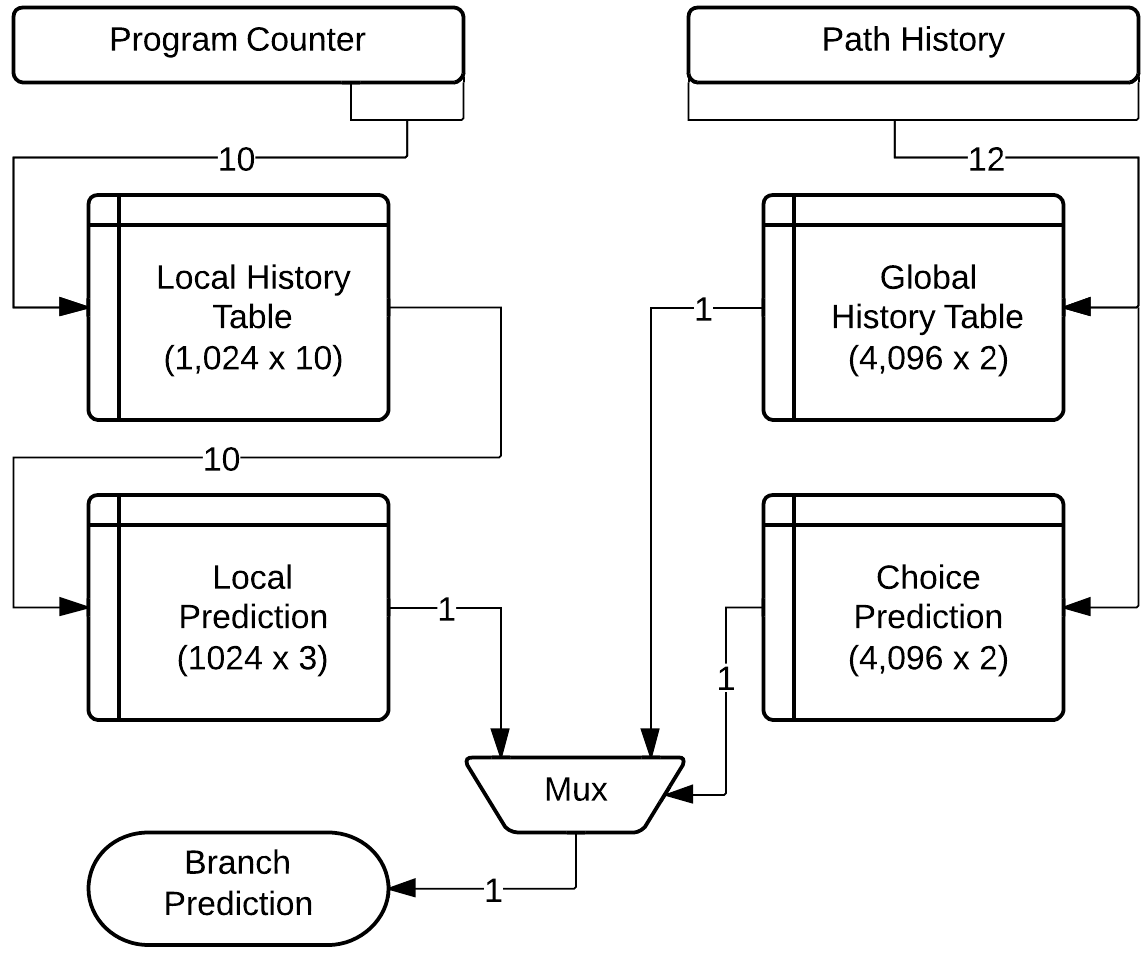
\includegraphics[width=\columnwidth]{img/alpha.png}}{Alpha Predictor}{alpha}\centerimage{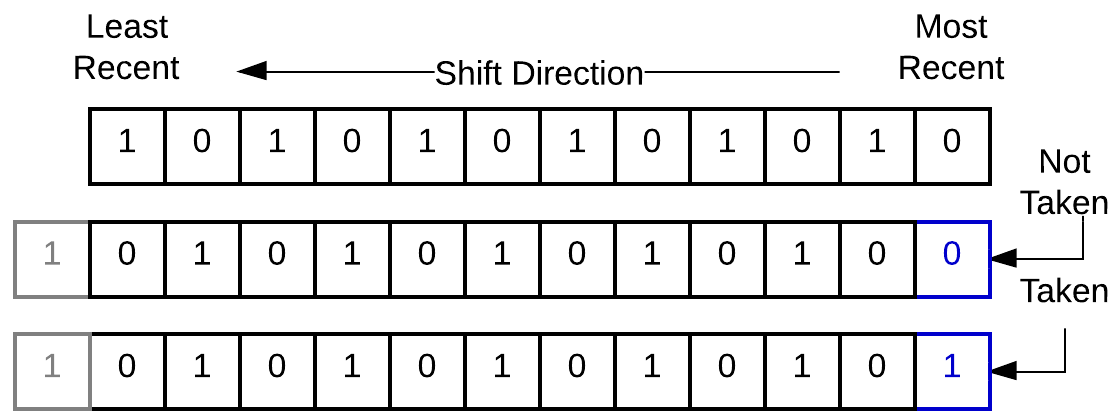
\includegraphics[width=\columnwidth]{img/phistory.png}}{Path History Shift Register}{phistory}
The Alpha predictor is a tournament predictor, meaning that it makes multiple predictions (based on the global and local histories) and then chooses between the prediction that has  been the most accurate, based on the path history.  The path history (illustrated in figure \ref{phistory}) is a shift register that maintains a history of the most recent 12 conditional branches by shifting in 1 or 0 for taken or not taken branches respectively.\\\\
Path history is used as an index into the 4,096-entry choice prediction table, which maintains 2-bit saturating counters at each location which indicate whether--given the current path history--the local or global prediction has been more accurate.\\\\  
The global history table is also indexed using the path history, and consists of 4,096 2-bit saturating counters indicating whether--given the current global path history--the next branch is likely to be taken or not taken.\\\\
The local history table is indexed by the least significant 10 bits of the program counter.  Each entry in the local history table is a 10-bit path history for instructions (in our implementation, \textit{conditional branches}) with the same least significant 10 bits.  These local histories are used as indices into the local prediction table, which consists of 1,024 3-bit saturating counters indicating whether--given a local path history--the next branch is likely to be taken or not taken.\\\\
The strength of this design is that it can take advantage of branch patterns occurring within working sets of various sizes, with the local history being more useful with small working sets, and the global history being more useful for large working set.\\\\
A few implementation details were absent from Kessler's paper, so assumptions were made to create the most accurate predictor possible.  These fell into three categories:  Initialization values for the saturating counters and path history, under what conditions updates should occur, and how to handle unconditional branches (jumps).

\subsection{Initialization Values}
To start, we initialized everything to zero. This was to verify that our logic was working correctly. After verifying that things looked like they were working, we decided to see if tuning these parameters would have a major effect on our performance. Zeros would imply that our default state should be strongly not taken for both the local and global predictors, and strongly favoring the local predictor for the predictor predictor.\\\\
For an initial state, neither strongly taken nor strongly not taken are useful, as there is no previous state to base this off. Instead, it follows that being on the cusp of either state. We determined that for the traces used, weakly not taken gives better peformance in general. Also, for the predictor predictor, since there is no local history to draw from, it follows that relying on global history would be more useful, but allowing for local history predictions to quickly become the dominant predictions if they are being favored early. Therefore weakly global was used for the initial predictor predictor state. 
To demonstrate, figure blah demonstrates the average Alpha predictor mispredicts for strongly taken, strongly not taken, and weakly not taken (our value) for the Local predictor. 
\subsection{Conditional Updates}
\subsection{Unconditional Branches}

\section{Branch Target Prediction}
In a high-performance processor, simply predicting whether a branch is taken or not taken accurately is not enough to eliminate pipeline stalls.  If taken, the destination address of the branch must also be predicted so that instructions beginning at the target address can be speculatively executed. 
 
\subsection{Development History}
Our development process was much like a small weasel--somewhat iterative, yet dynamic and highly agile.  The space used for the branch predictor is 3,713 bytes (see table \ref{sizebudget} in Appendix A), meaning that any branch target predictor design had to fit in less than 4,382 bytes.
\subsubsection{Direct Mapped}
Our initial design centered around using as much of the remaining 4,382 bytes as possible to create a single, large direct-mapped cache with 1,024 entries, each storing a single 32-bit address, for a total size of 4,096 bytes.  This approach was appealing because of its extremely simple implementation, and because it eliminated the need to store tags for any of the data.  Tags are not needed because there was no guarantee that the data returned was ``correct'' so any aliasing simply results in in a misprediction, which though not helpful is not catastrophic. \\\\
Upon completing this design, initial simulations using the first 4 trace files (FP-1, INT-1, MM-1, SERV-1) confirmed that aliasing was indeed a much larger problem than we had anticipated.

\subsubsection{Relative Offset Table}
In order to fit ``more cache'' into the available space, we redesigned the large cache from 3.1.1 to operate only on PC-relative branches, and only store the offset from the PC, which was only 24 bits.  This reduced the size of the table by 25\% to 3,072 bytes.  We had planned on using the additional 1024 bytes freed to create a smaller, wider cache that could store full 32-bit addresses that could not fit into the relative offset cache, however again, the amount of aliasing--even when considering only PC-relative branches--was far too high.\\\\
The smaller, 32-bit wide cache was never implemented because of the amount of aliasing that occurred with direct mapped caches, even when we increased the cache to be unrealistically large. 

\subsection{Final Design}
Our final design abandoned all direct-mapped tables and focused on multi-way associativity to reduce aliasing.  Our final design consisted of a large 512-entry main cache (64 sets x 8 ways), a 64-entry victim cache (8 sets x 8 ways), and a 33-entry return address stack to handle returns. 
\subsubsection{Dynamic Objects}
Very soon after the direct-mapped cache approach was abandoned, the decision was made to design all objects with dynamic sizes, so that we could easily experiment with differently sized caches with no code changes.  Parameterized LRU and Cache objects greatly accelerated all testing and simulation efforts. 
\subsubsection{Main Cache}
The main cache was given highest priority in terms of space allocation.  The bold entries in table \ref{sizebydim} (Appendix A) indicate the largest possible configurations we could accommodate while staying under 4,382 bytes.  Table \ref{mispersize} (Appendix A) shows the relative performance  of select cache configurations.\\\\
Looking at the results from tables \ref{sizebydim} and \ref{mispersize}, the 64-set x 8-way configuration resulted in the best performance under the size constraints of our project.  We also took note of the fact that a 128-set x 4-way had the second best performance but used over 100 bytes less space.  If a problem had arisen that an additional 100 bytes could have solved, we would have made this change, but ultimately this was unnecessary. 
\subsubsection{Victim Cache}
The victim cache was given second highest priority in terms of space allocation.  Since the primary purpose of the victim cache is to accommodate aliasing spillover, we wanted the maximum associativity possible given our available space.   After deciding to use the 64x8 main cache, we had 542 bytes of space remaining.  We referred again to table \ref{sizebydim} and selected the 8-sets x 8-ways cache, with a size of 504 bytes.  
\subsubsection{Return Address Stack}
The return address stack was much more flexible in terms of its size, since we were not limited to entry amounts that were powers of 2.  Hence, it was expanded to take up all of the remaining space, which yielded a 33-entry stack. 

\section{Size Budget}
\section{Testing Methodology}
\section{Results}
\section{Conclusion}
\appendix
\onecolumn
\section{Tables}
\vspace{-.15in}\centertable{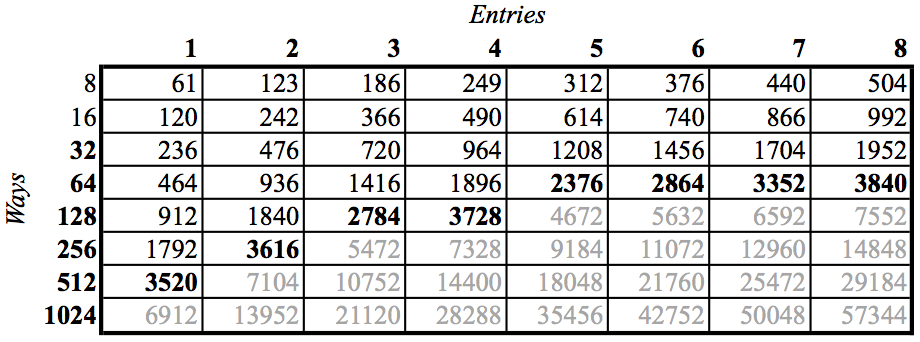
\includegraphics[width=5.25in]{img/sizebydim.png}}{Total space used (in bytes) for various cache dimensions}{sizebydim}
\vspace{-.35in}\centertable{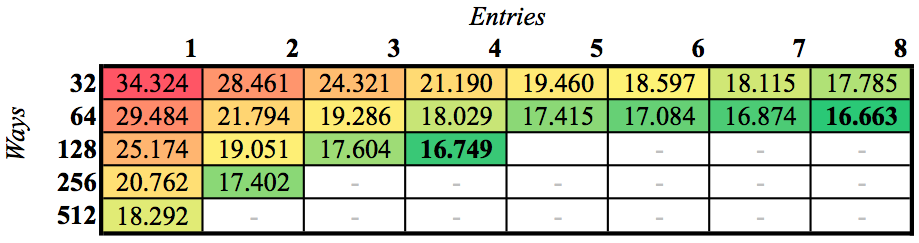
\includegraphics[width=5.25in]{img/mispersize.png}}{Target mispredictions/1000 instructions (Average of FP-1, INT-1, MM-1, and SERV-1 traces)}{mispersize}
\centertable{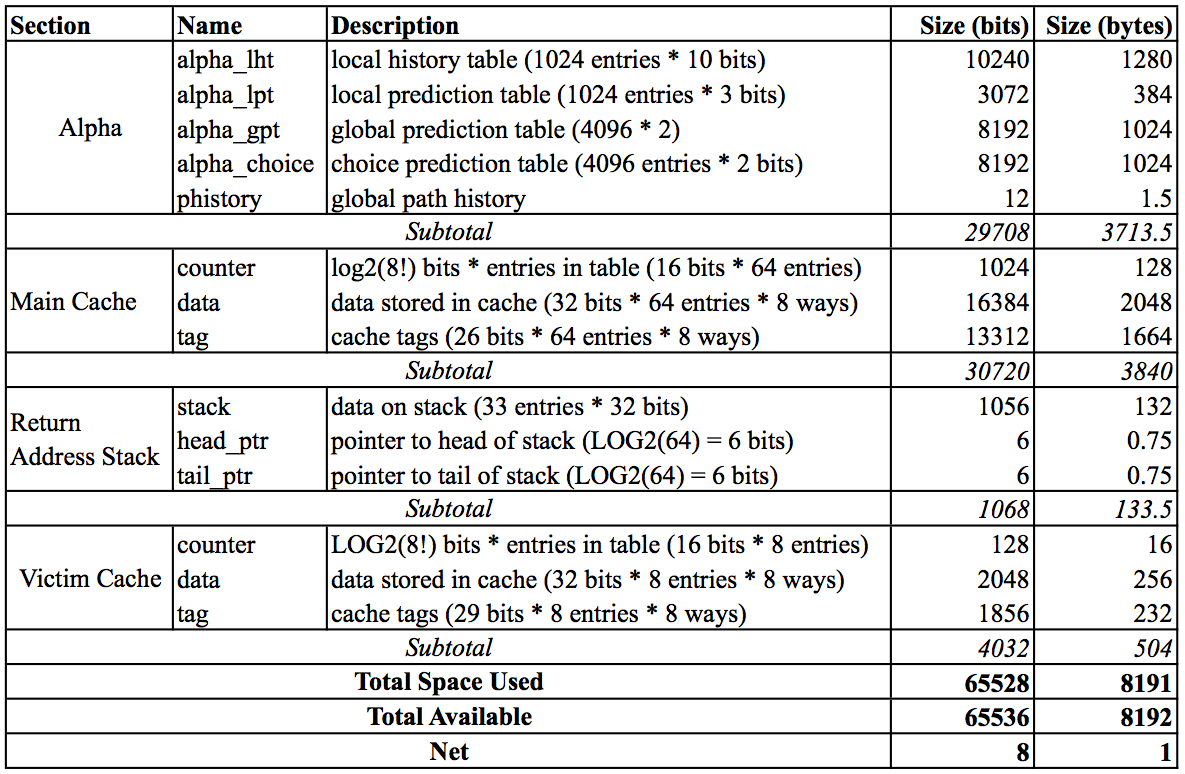
\includegraphics[width=\columnwidth]{img/sizebudget.png}}{Total size of all project elements}{sizebudget}
\end{document}
